\documentclass[11pt,a4paper]{article}
\usepackage[utf8]{inputenc}
\usepackage[french]{babel}
\usepackage[T1]{fontenc}
\usepackage{amsmath}
\usepackage{amsthm}
\theoremstyle{definition}
\newtheorem*{definition}{Definition}
\theoremstyle{remark}
\newtheorem*{remark}{Remark}
\usepackage{float}
\usepackage{amsfonts}
\usepackage{amssymb}
\usepackage{graphicx}
\usepackage{setspace}
\usepackage{gensymb} %Pour le degré
\usepackage{titlesec} %Pour le 3ème niveau de titres
\usepackage{fancyvrb} %Pour le Verbatim
\usepackage{alltt} %Environnement pseudo code
\usepackage{listings}% http://ctan.org/pkg/listings
\usepackage{listingsutf8}
\usepackage{geometry}
\lstset{
  basicstyle=\ttfamily,
  mathescape,
	literate={é}{{\'e}}1
           {è}{{\''e}}1
}
\lstinputlisting[inputencoding=utf8/latin1]

\newcommand{\reporttitle}{Rapport final}
\newcommand{\reportauthor}{Clément \textsc{Tamines} Jérémy \textsc{Gheysen}}
\newcommand{\reportsubject}{Projet de Structures de Données II}
\newcommand{\HRule}{\rule{\linewidth}{0.5mm}}
\renewcommand{\ttdefault}{txtt} %Pour le gras environnement pseudo-code

\setcounter{secnumdepth}{4}
\titleformat{\paragraph}
{\normalfont\normalsize\bfseries}{\theparagraph}{1em}{}
\titlespacing*{\paragraph}
{0pt}{3.25ex plus 1ex minus .2ex}{1.5ex plus .2ex}

\makeindex
\begin{document}
%TODO : Ajouter à la table des matières les paragraphes

%Page de garde
\begin{titlepage}
\begin{center}
\begin{minipage}[t]{0.48\textwidth}
  \begin{flushleft}
     
\includegraphics[width=42mm]{UMONS+txt.pdf} \\[0.5cm]
  \end{flushleft}
\end{minipage}
\begin{minipage}[t]{0.48\textwidth}
  \begin{flushright}
    
\includegraphics [width=42mm]{UMONS_FS.pdf} \\[0.5cm]
  \end{flushright}
\end{minipage} \\[1.5cm]

\vspace{1.5cm}
\textsc{\Large \reportsubject}\\[0.5cm]
\HRule \\[0.4cm]
{\huge \bfseries \reporttitle}\\[0.4cm]
\HRule \\[1.5cm]

\begin{minipage}[t]{0.3\textwidth}
  \begin{flushleft} \large
    \emph{Auteurs :}\\
    \reportauthor
  \end{flushleft}
\end{minipage}
\begin{minipage}[t]{0.6\textwidth}
  \begin{flushright} \large
    \emph{Professeur :} \\
    V. \textsc{Bruyère} \\
     \emph{Assistant :} \\
    G. \textsc{Devillez}
  \end{flushright}
\end{minipage}
\vfill
{\large 15 avril 2016}

\end{center}
\end{titlepage}

\tableofcontents
\newpage

\section*{Introduction}
\addcontentsline{toc}{section}{Introduction}
Ce projet consiste en l'implémentation d'un outil permettant, à partir d'un point de vue et d'une scène composée de segments colorés placés dans un repère orthonormé, d'afficher la scène telle que perçue par ce point de vue. Ce point de vue pourra être placé dans le repère par l'utilisateur.\\

Pour réaliser cet affichage, nous utiliserons l'algorithme du peintre tel que décrit dans le Chapitre 12 du livre \textit{Computational Geometry}. Cet algorithme s'applique sur des arbres qui stockent l'ensemble de segments qui compose la scène et qui permettent de trouver un ordre d'affichage correct pour un point de vue quelconque. Ces arbres sont appelés arbres BSP (\emph{Binary Spaces Partition}) et seront construit via différentes techniques à partir d'une liste de segments définis par leurs sommets et leur couleur. Nous présenterons dans ce rapport la technique \textit{in-order}, sa variante \textit{random} et le principe des \textit{free-splits}.\\

Ce rapport a pour but de décrire les différentes techniques et algorithmes utilisés lors de la construction des arbres BSP et de la visualisation de la scène à l'aide de l'algorithme du peintre. Nous analyserons également la complexité et la performance de ces algorithmes.

\newpage

\section{Arbres BSP}

\subsection{Principe}
Un arbre BSP (\emph{Binary Space Partition}), est un arbre binaire permettant de stocker de manière efficace un ensemble d'objets (dans notre cas de segments) situés dans un plan. Rappelons tout de même qu'un arbre binaire est un arbre tel que tout noeud possède au plus deux fils. \\

Le type d'arbre étudié ici consiste donc en une séparation binaire de l'espace, s'effectuant de manière récursive. Chaque noeud possède un ensemble de segments dans le plan et définit une nouvelle séparation binaire de ce dernier, cela sur base d'une droite (choisie selon une technique définie au préalable et dans laquelle sont contenus un ou plusieurs segments), et sépare ainsi le plan en deux sous-espaces contenant chacun une partie des segments restants. Cette méthode est alors appelée récursivement sur chacun des deux sous-espaces nouvellement créés (les deux fils) jusqu'au moment où tous les segments présents dans le plan sont contenus dans les noeuds de l'arbre. L'utilisation de la droite pour définir les nouveaux plans peut néanmoins couper des segments restants en deux, ces segments sont alors supprimés et les segments résultant de la coupure sont alors placés dans le fils leur correspondant en fonction de leur position. Remarquons qu'avec la manière avec laquelle nous définissons chaque nouveau noeud, les feuilles sont également des noeuds définissant deux nouveaux plans, mais ces derniers ne contiendront alors aucun segment (appel récursif alors impossible). \\

La taille d'un arbre BSP est calculée en fonction du nombre total de segments dans chacun de ses noeuds. Moins il y aura eu de fragmentation lors de la création de l'arbre, moins ce dernier aura de segments et donc moins il sera grand et inversément. Il est donc intéressant de limiter cette fragmentation. \\

Il existe bien évidemment diverses méthodes afin de construire de tels arbres de manière plus ou moins optimisée (en taille et/ou en temps), nous verrons ci-dessous trois de ces méthodes. 

Voici la définition récursive d'un arbre BSP que nous avons utilisé :

\theoremstyle{definition}
\begin{definition}{Arbre BSP}\\
\textit{Cas de base :} Un arbre BSP vide est un arbre BSP\\
\textit{Cas général :} Un arbre BSP est un composé d'un noeud contenant une ligne de séparation $s$, une liste chainée de segments contenus  dans cette ligne et une liste de segments dont ont doit déterminer si ils sont dans la séparation $s^+$ ou $s^-$. Il possède aussi deux fils qui sont eux-même des arbres BSP.
\end{definition}

\subsection{Éléments indispensables à la construction}

\subsubsection{Segment}
La classe Segment permet, comme son nom l'indique, de représenter un segment dans le plan orthonormé. Son constructeur prend en paramètres ses deux extrémités $(x1,y1)$, $(x2,y2)$ et sa couleur. Un segment possède également trois autres paramètres (\emph{intersected, isFreeSplit, intersection}), nécessaires à l'implémentation de l'heuristique des free-splits. Nous nous attarderons sur ces éléments plus tard. \\
Ci-dessous sont présentées les méthodes les plus importantes pour la suite des calculs :
\begin{itemize}
\item \emph{computeLine} : Calcule l'équation de la droite générée à partir du segment en question sous la forme $ax + by + c = 0$;
\item \emph{getSide} : Cette méthode remplace les coordonnées $x$ et $y$ données en paramètres dans la droite également donnée en paramètre et retourne le résultat (donc 0 si le point est sur la droite);
\item \emph{computePosition} : Retourne la position relative du segment par rapport à la droite donnée en paramètre. Remarquons que pour cette méthode certaines conventions ont été prises. En effet, s'il y a intersection, cette dernière est retournée. Sinon, si le segment est à gauche de la droite, NaN est retourné, s'il est à droite, c'est Infinity qui est renvoyé. Notons également que si nous nous trouvons dans le cas où il y a intersection au niveau d'un sommet du segment, par facilité d'implémentation nous retournons NaN ou Infinity en fonction de sa position et non le point d'intersection. Car en effet, nous aurions sinon création d'un segment qui est en réalité un point lors de la création de l'arbre BSP (ce qui aurait consisté en une segmentation incorrecte). Ces différentes situations sont représentées dans la figure \ref{computePositionExample}
\end{itemize}

\subsubsection{BSPNode} 
Cette classe est utile pour le stockage des arbres BSP. Sa conception est très proche des structures utilisées pour la représentation de simples arbre binaire. Des adaptations ont uniquement été faites pour stocker dans chaque noeud le ou les segment(s) présent(s) dans la droite le caractérisant via une liste chainée, et une autre liste chainée pour les segments présents dans l'hyperplan défini par le père (tous les segments s'il s'agit de la racine). 

\subsection{Méthodes utiles}
Intersection angle, position, remplacement
\subsection{Construction}
\subsubsection{Heuristique "in-order"}

\paragraph{Méthode}

Cette heuristique est très intuitive et met simplement en pratique le principe des arbres BSP. Étudions son fonctionnement à l'aide de l'exemple représenté à la Figure \ref{scene_inordre} : 

\begin{figure}[!h]
\centering
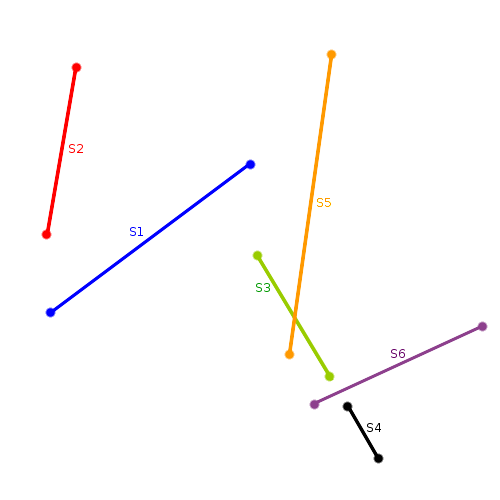
\includegraphics[scale=0.6]{bsp_ex_1.png}
\caption{Scène 2D}
\label{scene_inordre}
\end{figure}

Nous pouvons remarquer que cette scène contient 6 segments distincts, dont deux (les segments S3 et S4) se situant sur une même droite. Nous avons également des segments qui s'intersectent, ce qui va inexorablement mener à la création de nouveaux segments. Nous allons maintenant appliquer et expliquer le fonctionnement de l'heuristique "inordre", celui-ci étant représenté dans le plan à la Figure \ref{bsp_inordre} et l'arbre BSP correspondant est construit à la Figure \ref{bsp_tree}. \\

Cette heuristique travaille avec la liste des segments telle qu'elle a été fournie par l'utilisateur, c'est à dire que la création de l'arbre se fait dans l'ordre par lequel les segments ont été définis. \\

Nous commençons donc par une division du plan à l'aide de S1, et nous remarquons d'ores et déjà que S5 est alors coupé en deux segments S5A et S5B, en effet S5 intersecte la droite issue du prolongement de S1. Nous obtenons donc maintenant deux sous-ensembles de segments : 
$$S1^+ = \{S2, S5A\}$$
$$S1^- = \{S3,S4,S5B,S6\}$$

\begin{figure}[H]
\centering
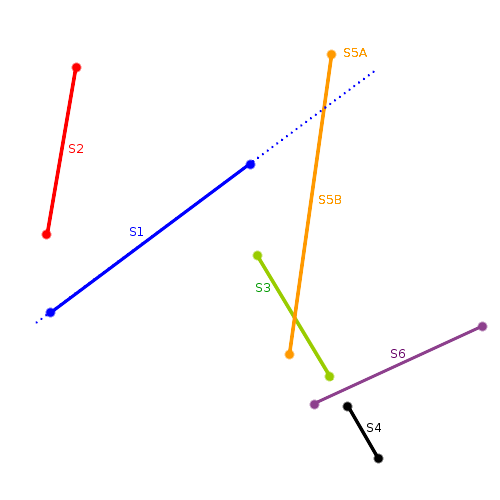
\includegraphics[scale=0.6]{bsp_ex_2.png}
\caption{Application de l'heuristique sur le noeud dont la droite est construire via $S_1$}
\label{bsp_inordre}
\end{figure}

Récursivement, l'algorithme va être appelé sur deux noeuds contenant les segments $S1^+$ et $S1^-$. Et c'est le premier segment de la liste qui sera utilisé comme nouvelle droite définissant les nouveaux plans. 
\begin{itemize}
\item Pour $S1^+$ on a donc ainsi $S_2$ comme segment de base pour la nouvelle droite. Il ne restera ainsi plus que $S5A$ comme feuille, comme indiqué sur la figure \ref{bsp_ex_4}.
\begin{figure}[H]
\centering
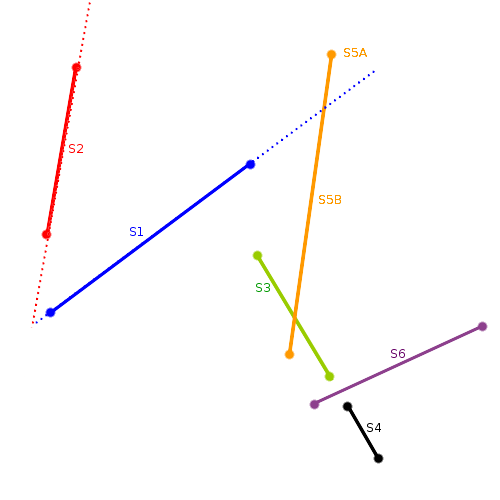
\includegraphics[scale=0.6]{bsp_ex_4.png}
\caption{Application de l'heuristique sur le noeud dont la droite est construire via $S_2$}
\label{bsp_ex_4}
\end{figure}

\item Pour $S1^-$ on a $S_3$ comme origine de la nouvelle droite et on remarque que $S_4$ est également inclu à la droite, donc ces deux segments font alors partie du même noeud. Nous avons également que $S_3$ intersecte $S5_B$ et $S_6$ ce qui engendre la création des segments : $S5_C$, $S6_A$, $S6_B$, la suppression du segment $S6$ et la modification de $S5_B$ (qui se traduira néanmoins techniquement par la suppression et la création d'un segment avec les coordonnées mises à jour) ceci est représenté à la figure \ref{bsp_ex_5}
\end{itemize}


\begin{figure}[H]
\centering
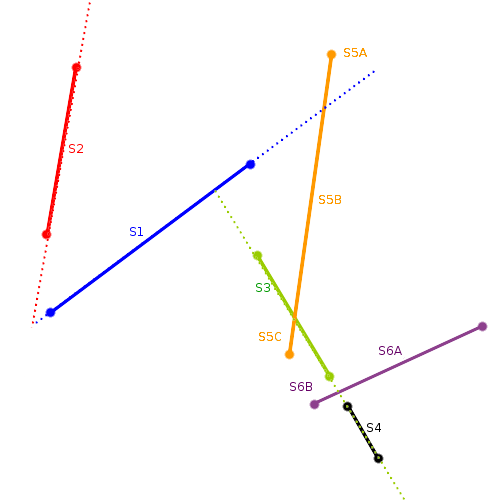
\includegraphics[scale=0.6]{bsp_ex_5.png}
\caption{Application de l'heuristique sur le noeud dont la droite est construire via $S_3$}
\label{bsp_ex_5}
\end{figure}

Suite aux appels récursifs, nous obtiendrons ainsi l'arbre suivant :

\begin{figure}[H]
\centering
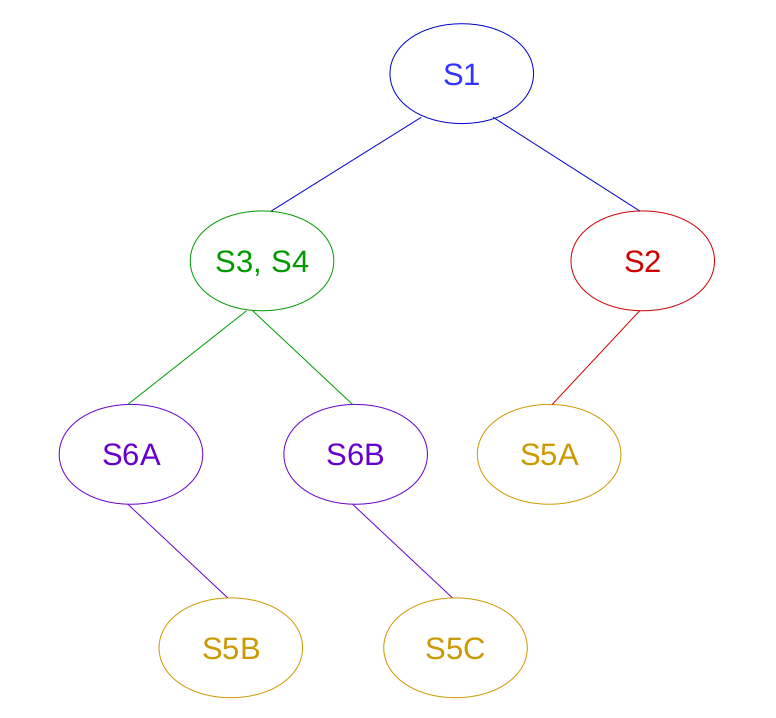
\includegraphics[scale=0.35]{bsp_ex_3.png}
\caption{Arbre BSP}
\label{bsp_tree}
\end{figure}

\paragraph{Implémentation}

Afin d'implémenter cette heuristique, nous utilisons principalement les 2 algorithmes suivants :
\begin{itemize}
\item createTree : permet de lancer la création de l'arbre;
\item createRoot : assure la construction récursive de l'arbre à partir d'un noeud;
\end{itemize}

Notons que nous utilisons les conventions suivantes :
\begin{itemize}
\item La création d'un noeud nécessite 4 paramètres : fils droit, fils gauche, la liste de segments de l'hyperplan et la droite effectuant la définition des deux nouveaux hyperplans (communément appelée "splitting line").
\item Un noeud possède 5 attributs : rightSon, leftSon, segmentsInHyperplane (liste des segments dans l'hyperplan défini par le droite de séparation du père), segmentsInLine (segments dans la ligne de séparation), line (tableau de trois doubles étant les facteurs a, b et c de l'équation de sa droite de séparation).
\item Un noeud possède entre autres les deux méthodes setLeftSon et setRightSon permettant d'ajouter respectivement un fils gauche et/ou un fils droit au noeud. 
\end{itemize}

\begin{alltt}
\textbf{createTree}
Entrée : segList, liste de segments d'origine pour la création 
de l'arbre BSP
Sortie : racine de l'arbre BSP généré

1: \(line \leftarrow segList[0]\)
2: enlever \(segList[0]\) de \(segList\)
3: \(racine\) \(\leftarrow\) nouveau noeud (\(vide\), \(vide\), \(segList\), \(line\))
4: createRoot(\(racine\))
5: retourner \(racine\)
\end{alltt}

\begin{alltt}
\textbf{createRoot}
Entrée : noeud, étant un noeud incomplet de l'arbre BSP ne
disposant que de sa ligne de séparation et sa liste de
segments contenus dans son hyperplan.
Sortie : /
Effet : ajoute les fils au noeud s'il en a et dans ce cas 
appelle l'algorithme récursivement sur ces derniers en 
choisissant une nouvelle droite de séparation et en 
donnant les nouvelles listes de segments adaptées.

 1: si \(noeud\) non vide alors
 2:   pour chaque segment \(s\) dans \(noeud.segmentsInHyperplane\) faire
 3:     si \(s \in noeud.line\) alors
 4:       ajouter \(s\) à \(segmentsInLine\)
 5:       enlever \(s\) de \(segmentsInHyperplane\)
 6:       
 7:   créer les listes \(leftNodeSegments\) et \(rightNodeSegments\)
 8:   
 9:   pour chaque segment \(s\) dans \(noeud.segmentsInHyperplane\) faire
10:     si \(s\) est à droite de \(noeud.line\) alors
11:       ajouter \(s\) à \(rightNodeSegments\)
12:
13:     sinon si \(s\) est à gauche de \(noeud.line\) alors
14:       ajouter \(s\) à \(leftNodeSegments\)
15:
16:     sinon on est dans le cas où \(s\) intersecte \(noeud.line\) alors
17:       créer deux nouveaux segments \(s1\) et \(s2\)
18:       si \(s1\) est à droite de \(noeud.line\) alors
19:         ajouter \(s1\) à \(rightNodeSegments\)
20:         ajouter \(s2\) à \(leftNodeSegments\)
21:
22:       sinon
23:         ajouter \(s1\) à \(leftNodeSegments\)
24:         ajouter \(s2\) à \(rightNodeSegments\)
25:         
26:   si \(leftNodeSegments\) et \(rightNodeSegments\) sont non-vides alors
27:     \(line \leftarrow rightNodeSegments[0]\)
28:     enlever \(rightNodeSegments[0]\) de \(rightNodeSegments\)
29:     \(rightNode \leftarrow\) nouveau noeud (\(vide\), \(vide\), \(rightNodeSegments\), \(line\))
30:     setRightSon(\(rightNode\))
31:     \(line \leftarrow leftNodeSegments[0]\)
32:     enlever \(leftNodeSegments[0]\) de \(leftNodeSegments\)
33:     \(leftNode \leftarrow\) nouveau noeud (\(vide\), \(vide\), \(leftNodeSegments\), \(line\))
34:     setLeftSon(\(leftNode\));
35:     
36:   sinon si \(leftNodeSegments\) vide et \(rightNodeSegments\) non-vide alors
37:     \(line \leftarrow rightNodeSegments[0]\)
38:     enlever \(rightNodeSegments[0]\) de \(rightNodeSegments\)
39:     \(rightNode \leftarrow \) nouveau noeud (\(vide\), \(vide\), \(rightNodeSegments\), \(line\))
40:     setRightSon(\(rightNode\))
41:    
42:   sinon si \(leftNodeSegments\) non-vide et \(rightNodeSegments\) vide alors
43:     \(line \leftarrow leftNodeSegments[0]\)
44:     enlever \(leftNodeSegments[0]\) de \(leftNodeSegments\)
45:     \(leftNode \leftarrow \) nouveau noeud (\(vide\), \(vide\), \(leftNodeSegments\), \(line\))
46:     setLeftSon(\(leftNode\))
47:     
48:   createRoot(\(leftNode)\))
49:   createRoot(\(rightNode\))
\end{alltt}

Pour effectuer la création d'un arbre BSP avec l'heuristique "inordre" nous appelons simplement createTree avec la liste des segments devant former l'arbre. Cet algortihme va alors se charger d'initialiser le premier noeud en utilisant le premier segment de la liste comme droite de séparation. Ensuite l'algorithme createRoot est appelé avec ce premier noeud, c'est cet algorithme qui se charge ensuite de la construction récursive de l'arbre. \\

Tout d'abord, l'instruction 1 permet de ne faire fonctionner l'algorithme que s'il a du sens, c'est à dire que le noeud sur lequel il est appelé est non nul. Nous pouvons ensuite effectuer une analyse en deux parties : 

La première partie, constituée des instructions 2 à 25, consiste en la création de deux nouveaux hyperplans $s^+$ et $s^-$ en fonction de la "splitting line", ou droite de division de l'espace $s$ du noeud. On regarde d'abord si des segments de l'hyperplan du noeud sont contenus dans cette droite et, s'ils existent, on les ajoute à la liste des segments contenus dans la droite. Ensuite, avec les segments restants, on va regarder s'ils se situent à gauche ou à droite de la "splitting line", donc $s^+$ ou $s^-$ pour ensuite pouvoir les répartir correctement (dans le cas où il y a intersection, on crée deux nouveaux segments et on les ajoute au bon nouvel hyperplan en fonction de leur position). 

La seconde partie permet la création de la structure d'arbre en tant que tel, constituée des instructions 26 à 49. Elle va simplement attribuer au noeud un fils gauche et un fils droit si de tels fils existent. En effet, on peut se trouver dans le cas d'une feuille, ou on a juste un ou plusieurs segments dans $segmentsInLine$ qui définissent une "`splitting line"' mais aucuns segments dans "`segmentsInHyperPlane". Nous pouvons aussi nous trouver dans le cas ou il n'y a aucun segment compris dans $s^+$ ou $s^-$, ce qui revient à ne pas avoir de fils droit ou gauche. L'hyperplan correspondant au noeud, calculé dans la première partie, leur est attribué et une nouvelle droite de séparation (générée à partir du premier segment de l'hyperplan) leur est donnée. Ensuite l'algorithme est appelé récursivement sur ces deux fils (pouvant résulter sur un appel récursif sur un fils Null qui sera écartée par l'instruction 1. 

\paragraph{Complexité}

\subsubsection{Heuristique "random"}

\paragraph{Méthode}

Cette heuristique utilise la même méthode que l'heuristique "inordre" pour la création de l'arbre BSP, à la seule différence près que la liste des segments est mélangée avant de commencer la construction. La différence d'un point de vue algorithmique avec l'heuristique précédente étant nulle, nous ne attardons donc pas sur ce point. 

\paragraph{Implémentation}

L'implémentation de cette heuristique est identique à la précédente à l'exception d'une ligne effectuant le mélange de la liste des segments avant utilisation. On va donc ici mélanger la liste des segments, puis appeler l'algorithme précédent :

\begin{alltt}
\textbf{createTree}
Entrée : segList, liste de segments d'origine pour la création 
de l'arbre BSP
Sortie : racine de l'arbre BSP généré

1: \(inorder \leftarrow\) nouveau InOrderHeuristic()
2: mélanger \(segList\)
3: retourner inorder.createTree(\(segList\))
\end{alltt}

\paragraph{Complexité}

N'ayant effectué qu'un mélange de liste en \emph{O(n)} en dehors de toute boucle ou appel récursif, cela n'aucun impact au niveau de la complexité asymptotique. 

\subsubsection{Heuristique "free-splits"}

\paragraph{Méthode}

Afin d'expliquer au mieux cette heuristique, nous utiliserons également un exemple, représenté à la Figure \ref{scene_splits}. \\

Cette heuristique se veut plus réfléchie que la simple utilisation, dans un ordre aléatoire ou non, des segments pour la définition de nouveaux plans. Nous allons donc étudier ici le cas particulier des "free-splits", ce dernier n'apparaissant que dans des circonstances bien précises, recréées ici dans l'exemple. Notons que cette heuristique se base sur une liste de segments ordonnés de manière aléatoire, néanmoins, pour les besoins de l'exemple nous supposerons que l'algorithme traite les segments dans l'ordre où ceux-ci ont été définis. En effet, si nous traitons les segments dans un ordre aléatoire, il se pourrait que nous soyons en présence d'une situation ne disposant pas de "free-split".

\begin{figure}[!h]
\centering
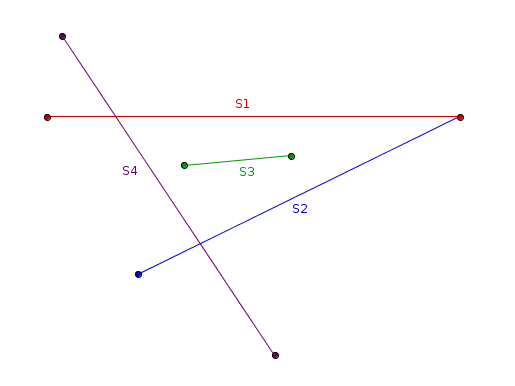
\includegraphics[scale=0.5]{free_splits_2.png}
\caption{Scène 2D}
\label{scene_splits}
\end{figure}

Exécutons pas à pas l'algorithme et définissons à l'aide de l'exemple la notion de "free-split". \\

Nous pouvons observer que cette scène est composée de 4 segments. Imaginons que nous avons déjà construit une partie de l'arbre BSP avec S1 et S2, nous remarquons alors que ces deux segments coupent S4, ce qui divise S4 en trois nouveaux segments (nommés S4A, S4B et S4C dans la Figure \ref{heuristic_splits}). A cette étape nous avons déjà la partie gauche de l'arbre construite avec S4A en tant que feuille (voir Figure \ref{split_bsp}). Il reste alors à construire le côté droit à partir de S2. S4C étant tout seul de son côté, le choix se porte alors entre S3 et S4B comme base pour une nouvelle droite. Or étant donné que S4B est déjà intersecté par deux droites, l'utiliser comme nouvelle droite ne causera pas de nouvelle fragmentation lors de la création du noeud ! C'est ce que l'on appelle la notion de "free-splits", c'est à dire utiliser des segments déjà intersectés par deux droites existantes pour définir de nouveaux plans, car ceux-ci, par conséquent ne fragmenteront plus aucun segment. Ce qui donc est avantageux au niveau de la quantité de segments qui est alors censée être réduite.\\

Notons que lorsqu'aucun "free-split" n'est présent, c'est l'algorithme classique "random" de création d'arbre BSP qui est d'application. 

\begin{figure}[!h]
\centering
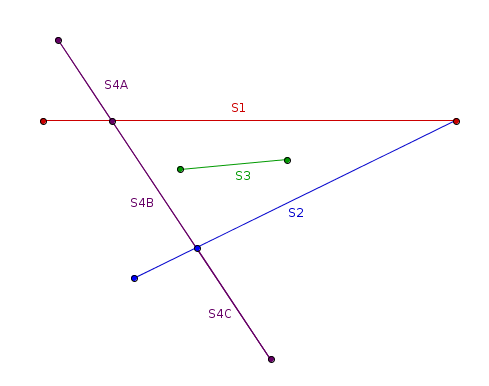
\includegraphics[scale=0.5]{free_splits_1.png}
\caption{Application de l'heuristique}
\label{heuristic_splits}
\end{figure}


\begin{figure}[!h]
\centering
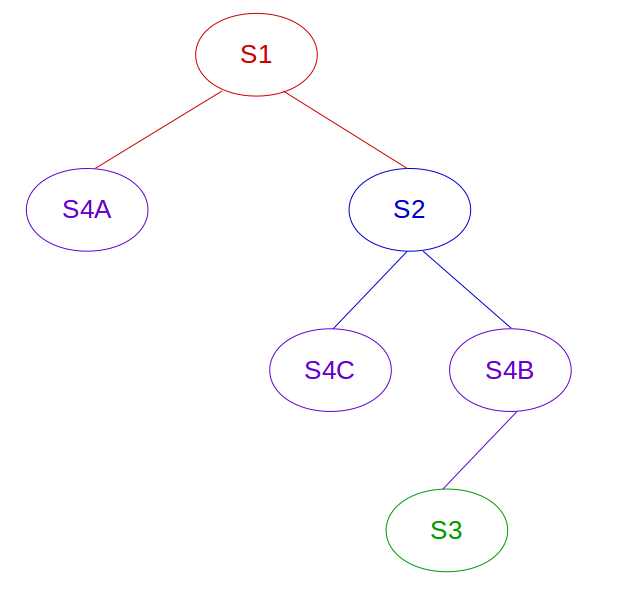
\includegraphics[scale=0.4]{free_splits_3.png}
\caption{Arbre BSP}
\label{split_bsp}
\end{figure}

\paragraph{Implémentation}

L'implémentation de l'heuristique des "free-splits" paraît à première vue fort semblable par rapport à celle "inorder", ce qui est normal étant donné qu'elles possèdent le même squelette, "free-splits" n'apportant que quelques améliorations se basant sur des conditions supplémentaires. Nous allons donc ici présenter un pseudo-code très semblable au précédent, c'est pourquoi les numéros de lignes présentant un changement seront mises en gras.\\

Pour les besoins de l'heuristique nous introduisons les attributs suivants aux objets de type segment : un booléen isIntersected indiquand si le segment a déjà été intersecté ou non, un tableau de deux nombres nommé intersection contenant cette intersection si elle existe et un booléen isFreeSplit indiquant si le segment est un "free-split". Notons également les deux abréviations suivantes : a et b pour désigner les deux extrémités du segment.\\

Notons bien qu'afin de comprendre sans ambiguïté les lignes 20,25,27 et 30, nous admettons que lorsque nous réalisons une coupure au niveau d'un segment par une droite, celle-ci se fait au niveau de l'extrémité b pour les nouveaux segments. 

\begin{alltt}
\textbf{createTree}
Entrée : segList, liste de segments d'origine pour la création 
de l'arbre BSP
Sortie : racine de l'arbre BSP généré

\textbf{1:} mélanger \(segList\)
2: \(line \leftarrow segList[0]\)
3: enlever \(segList[0]\) de \(segList\)
4: \(racine\) \(\leftarrow\) nouveau noeud (\(vide\), \(vide\), \(segList\), \(line\))
5: createRoot(\(racine\))
6: retourner \(racine\)
\end{alltt} 

\begin{alltt}
\textbf{createRoot}
Entrée : noeud, étant un noeud incomplet de l'arbre BSP ne
disposant que de sa ligne de séparation et sa liste de
segments contenus dans son hyperplan.
Sortie : /
Effet : ajoute les fils au noeud s'il en a et dans ce cas 
appelle l'algorithme récursivement sur ces derniers en 
choisissant une nouvelle droite de séparation et en 
donnant les nouvelles listes de segments adaptées.

 1: si \(noeud\) non vide alors
 2:   pour chaque segment \(s\) dans \(noeud.segmentsInHyperplane\) faire
 3:     si \(s \in noeud.line\) alors
 4:       ajouter \(s\) à \(segmentsInLine\)
 5:       enlever \(s\) de \(segmentsInHyperplane\)
 6:       
 7:   créer les listes \(leftNodeSegments\) et \(rightNodeSegments\)
 8:   
 9:   pour chaque segment \(s\) dans \(noeud.segmentsInHyperplane\) faire
10:     si \(s\) est à droite de \(noeud.line\) alors
11:       ajouter \(s\) à \(rightNodeSegments\)
12:
13:     sinon si \(s\) est à gauche de \(noeud.line\) alors
14:       ajouter \(s\) à \(leftNodeSegments\)
15:
16:     sinon on est dans le cas où \(s\) intersecte \(noeud.line\) alors
17:       créer deux nouveaux segments \(s1\) et \(s2\)
18:
\textbf{20:}		      si \(s\) est intersecté et intersection \(=s1.a\) alors
\textbf{21:}		        \(s1\) devient un free-split
\textbf{22:}		    
\textbf{23:}		      sinon
\textbf{24:}		        \(s1\) devient intersecté
\textbf{25:}		        \(s1.intersection\) = \(s1.b\)
\textbf{26:}		    
\textbf{27:}		      si \(s\) est intersecté et intersection \(=s2.a\) alors
\textbf{28:}		        \(s2\) devient un free-split
\textbf{29:}		    
\textbf{30:}		      sinon
\textbf{31:}		        \(s2\) devient intersecté
\textbf{32:}		        \(s2.intersection\) = \(s2.b\)
33:		
34:       si \(s1\) est à droite de \(noeud.line\) alors
35:         ajouter \(s1\) à \(rightNodeSegments\)
36:         ajouter \(s2\) à \(leftNodeSegments\)
37:
38:       sinon
39:         ajouter \(s1\) à \(leftNodeSegments\)
40:         ajouter \(s2\) à \(rightNodeSegments\)
41:   
\textbf{42:}	  \(fsLeft = faux\)
\textbf{43:}	  \(fsRight = faux\)
\textbf{44:}      
\textbf{45:}   si taille de \(leftNodeSegments < 1\)
\textbf{46:}     pour chaque segment \(s\) dans \(leftNodeSegments\) faire
\textbf{47:}       si \(s\) est free-split
\textbf{48:}         \(fsLeft = true\)
\textbf{49:}         enlever \(s\) de \(leftNodeSegments\)
\textbf{50:}         \(leftNode \leftarrow \) nouveau noeud (\(vide\), \(vide\), \(leftNodeSegments\), \(s\))
\textbf{51:}         setLeftSon(\(leftNode\))
\textbf{52:}            
\textbf{53:}    si taille de \(rightNodeSegments < 1\)
\textbf{54:}      pour chaque segment \(s\) dans \(rightNodeSegments\) faire
\textbf{55:}        si \(s\) est free-split
\textbf{56:}          \(right = true\)
\textbf{57:}          enlever \(s\) de \(rightNodeSegments\)
\textbf{58:}          \(rightNode \leftarrow \) nouveau noeud (\(vide\), \(vide\), \(rightNodeSegments\), \(s\))
\textbf{59:}          setrightSon(\(rightNode\))
60:
61:   si \(leftNodeSegments\) et \(rightNodeSegments\) sont non-vides alors
\textbf{62:}	    si \(fsRight\) est faux
63:       \(line \leftarrow rightNodeSegments[0]\)
64:       enlever \(rightNodeSegments[0]\) de \(rightNodeSegments\)
65:       \(rightNode \leftarrow\) nouveau noeud (\(vide\), \(vide\), \(rightNodeSegments\), \(line\))
66:       setRightSon(\(rightNode\))
67
\textbf{68:}	    si \(fsLeft\) est faux
69:       \(line \leftarrow leftNodeSegments[0]\)
70:       enlever \(leftNodeSegments[0]\) de \(leftNodeSegments\)
71:       \(leftNode \leftarrow\) nouveau noeud (\(vide\), \(vide\), \(leftNodeSegments\), \(line\))
72:       setLeftSon(\(leftNode\));
73:     
\textbf{74:}   sinon si \(leftNodeSegments\) vide et \(rightNodeSegments\) non-vide et
\textbf{75:}   \(fsLeft\) est faux alors
76:     \(line \leftarrow rightNodeSegments[0]\)
77:     enlever \(rightNodeSegments[0]\) de \(rightNodeSegments\)
78:     \(rightNode \leftarrow \) nouveau noeud (\(vide\), \(vide\), \(rightNodeSegments\), \(line\))
79:     setRightSon(\(rightNode\))
80:    
\textbf{81:}   sinon si \(leftNodeSegments\) non-vide et \(rightNodeSegments\) vide 
\textbf{82:}   et \(fsRight\) est faux alors
83:     \(line \leftarrow leftNodeSegments[0]\)
84:     enlever \(leftNodeSegments[0]\) de \(leftNodeSegments\)
85:     \(leftNode \leftarrow \) nouveau noeud (\(vide\), \(vide\), \(leftNodeSegments\), \(line\))
86:     setLeftSon(\(leftNode\))
87:     
88:   createRoot(\(leftNode)\))
89:   createRoot(\(rightNode\))
\end{alltt}

Au niveau du code présent aux lignes 20-32, il s'agit de la recherche de free-splits. En effet ceux-ci peuvent se créer lorsqu'il y a une coupure d'un segment par une droite. Ce dernier, si déjà intersecté précédemment, présente alors un free-split sur un de ses sous-segments récemment créés. C'est ce que nous réalisons aux lignes 20-21 et 27-28, en vérifiant bien si nous nous trouvons sur le bon sous-segment. Par contre si le segment original n'a pas encore été intersecté, nous marquons les deux sous-segments comme intersectés et conservons dans une variable le point d'intersection. \\

Pour les instructions 42-59, il s'agit simplement d'une vérification permettant de savoir si des free-splits sont présent dans la liste des segments pour le fils gauche et le fils droit. Si c'est le cas, le noeud est créé avec le segment résultant du free-split comme base pour une nouvelle droite de séparation, un booléen est mis à vrai et il n'y aura donc pas de choix aléatoire comme dans l'heuristique précédente. Et cela grâce aux conditions ajoutée en 62,68,74-75 et 81-82. Si aucun free-split n'est trouvé, le premier segment de l'hyperplan en question est choisi comme nouvelle "splitting-line", comme dans l'heuristique précédente. 

\subsection{Complexité}

\subsection{Structures de données utilisées}
Outre nos structures de données pour représenter les arbres BSP, nous avont fait le choix d'utiliser des listes chainées de Java contenir les segments (que ce soient les segments contenus dans la ligne de séparation $s$ ou ceux compris dans les séparations de l'espace $s^+$ et $s^-$). 
L'avantage de ces structures de données est la récupération du premier élément et sa suppression en O(1). En effet, une référence au début de la liste étant toujours gardée, il est très peu couteux d'y accéder et de la supprimer. Etant donné que les segments sont traités dans l'ordre de la liste dans le but de créer une ligne de séparation $s$, il est intéressant de pouvoir facilement accéder au premier segment. 
Dans un second temps, il est utile de remarquer que l'ajout d'un segment dans une liste chainée se fait aussi en O(1) via l'utilisation d'une référence au dernier élément de la liste. Ceci est très utile vu que des segments sont ajouté à des listes chainées constamment (que ce soit un segment qui se trouve dans $s^+$ ou $s^-$ et qui doit donc être placé dans la liste chainée correspondante ou que ce soit les fragments ajoutés à ces listes suite à la coupure d'un segment).

\subsection{Tests \& Résultats}

Dans cette section nous allons analyser les performances des différentes heurisitiques pour la création des arbres BSP. \\

\section{Algorithme du peintre}

Notre implémentation de l'algorithme du peintre est similaire à celle présentée dans le livre de référence. Son principe est le suivant : chaque noeud de l'arbre BSP est parcouru dans un certain ordre et les segments qu'il contient sont alors affichés.

\subsection{Algorithme principal}
\subsubsection{Pseudo-code}
\begin{lstlisting}
paintersAlgorithm
Entrées : N la racine d'un arbre BSP, P un point de vue
Sortie : / (les segments sont dessinés dans le bon ordre)

 1: si !vide(N) alors
 2
 3:    si feuille(N) alors
 4:       drawSegments($N_{liste}$)
 5:
 6:    si $P \in N_{s^+}$ alors
 7:       paintersAlgorithm($N_{filsGauche}$,$P$)
 8:       drawSegments($N_{liste}$)
 9:       paintersAlgorithm($N_{filsDroit}$,$P$)
10:
11:    si $P \in N_{s^-}$ alors
12:       paintersAlgorithm($N_{filsDroit}$,$P$)
13:       drawSegments($N_{liste}$)
14:       paintersAlgorithm($N_{filsGauche}$,$P$)
15:
16:    sinon
16:       paintersAlgorithm($N_{filsDroit}$,$P$)
17:       paintersAlgorithm($N_{filsGauche}$,$P$)
\end{lstlisting}

\subsection{Complexité}
Nous remarquons tout d'abord que l'algorithme va parcourir tous les noeuds de l'arbre, la méthode scanConvert va quant à elle parcourir tous les segments contenus dans ces noeuds. Pour une entrée d'un arbre avec $n$ noeuds et $m$ segments, nous obtenons une complexité à un appel récursif $i_k$ telle quel O($i_k$) avec $i_1 + i_2 + ... + i_k + ... + i_n$ =$m$. On a donc pour les n noeuds une complexité en 


\subsubsection{Explications}
Cet algorithme permet de parcourir l'arbre BSP pour afficher les segments par ordre de distance avec le point de vue (les segments les plus éloignés étant dessinés en premier).
Nous vérifions tout d'abord si la racine de l'arbre N n'est pas vide, ceci peut résulter d'un appel récursif sur l'algorithme avec un noeud $N$ qui n'a pas de fils gauche ou droit. L'appel se fera donc avec un noeud null et ne résultera en aucun calcul.

Ensuite, il est évident que si le noeud $N^$ est une feuille, nous ne pouvons plus parcourir récursivement l'arbre et nous appellons la méthode qui permet d'afficher les segments contenus dans le noeud $N$ via $N_{liste}$. Cette méthode déterminera si ces segments sont compris dans la vue et les dessinera le cas échéant.

Si le point de vue $P$ appartient à $N_{s^+}$, nous nous voulons d'abord afficher les segments plus distants que ceux de $N_{liste}$, 
ceux si seront ceux du fils gauche qui appartient à $N_{s^-}$ et possède donc des segments plus distants du point de vue comme détaillé sur la figure \ref{ordre_1}. Le même principe s'applique pour le cas ou $P$ appartient à $N_{s^-}$.

\begin{figure}[!h]
\centering
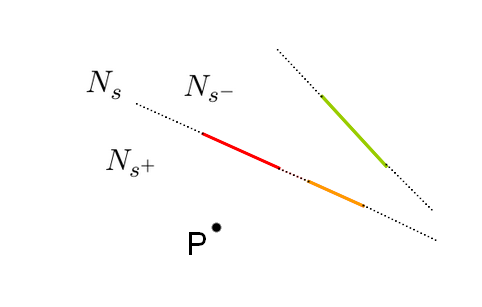
\includegraphics[scale=0.5]{painter_ordre_1.png}
\caption{Ordre de parcours si $P \in N_{s^+}$ }
\label{ordre_1}
\end{figure}

Si $P$ n'appartient pas à $N_{s^+}$ ni à $N_{s^-}$ alors $P \in N_s$ et les segments du noeud $N$ ne doivent pas être affichés et le parcours est continué.

\subsection{Algorithme de projection}

\subsubsection{Pseudo-code}

\begin{lstlisting}
drawSegments
Entrées : L une liste d'objets segments
Sortie : / (les segments sont dessinés via l'objet g2)
\end{lstlisting}

Les figure \ref{painter_notations} et \ref{painter_notations_2} rend compte des notations utilisées dans l'algorithme.
\\
\begin{figure}[!htbp]
  \centering
  \begin{minipage}[b]{0.4\textwidth}
    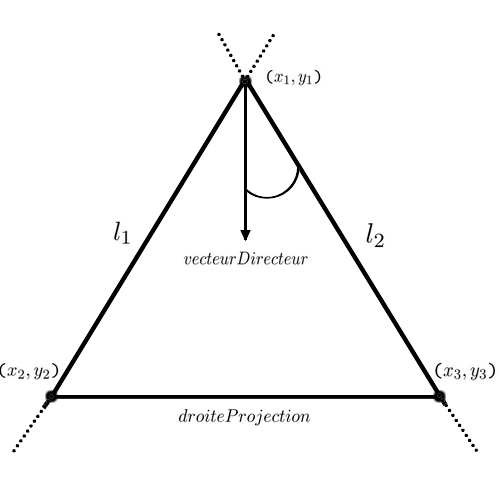
\includegraphics[width=\textwidth]{painter_notations.png}
    \caption{Notations du point de vue}
		\label{painter_notations}
  \end{minipage}
  \hfill
  \begin{minipage}[b]{0.4\textwidth}
    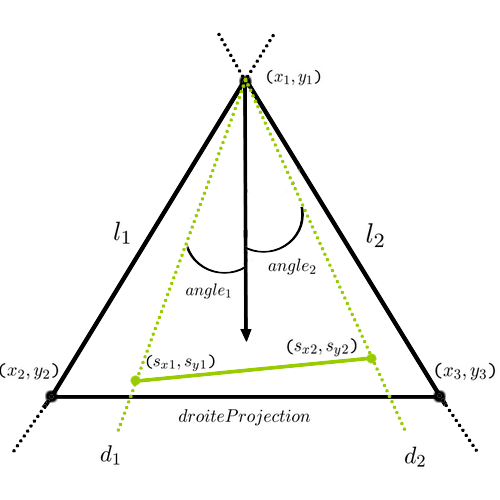
\includegraphics[width=\textwidth]{painter_notations_2.png}
    \caption{Notations avec segment $s$}
		\label{painter_notations_2}
  \end{minipage}
\end{figure}
\\

\newpage

\newgeometry{margin=0.4in}
\begin{lstlisting}
 1: $l_1$ $\leftarrow$ calcDroite($x_1,y_1,x_2,y_2$)
 2: $l_2$ $\leftarrow$ calcDroite($x_1,y_1,x_3,y_3$)
 3: $limite_1$ $\leftarrow$ ($x_2,y_2$)
 4: $limite_2$ $\leftarrow$ ($x_3,y_3$)
 5: $position$ $\leftarrow$ ($x_1,y_1$)
 6: $vecteurDirecteur$ $\leftarrow$ pointDeVue.vecteurDirecteur
 7: $demisAngle$ $\leftarrow$ calcAngle($l_1$, $vecteurDirecteur$)
 8: $droiteProjection$ $\leftarrow$ calcDroite($x_2,y_2,x_3,y_3$)
 9: 
10: pour chaque segment $s$ dans $L$ faire
11:   $d_1$ $\leftarrow$ calcDroite($x_1,y_1,s_x_1,s_y_1$)
12:   $d_2$ $\leftarrow$ calcDroite($x_1,y_1,s_x_2,s_y_2$)
13:   $angle_1$ $\leftarrow$ calcAngle($vecteurDirecteur$, $d_1$)
14:   $angle_2$ $\leftarrow$ calcAngle($vecteurDirecteur$, $d_2$)
15:
16:   si $|angle_1| \leq |demisAngle|$ et $|angle_2| \leq |demisAngle|$ alors
17:      $i_1$ $\leftarrow$ calcInter($d_1$,$droiteProjection$)
17:      $i_2$ $\leftarrow$ calcInter($d_2$,$droiteProjection$)
18:      dessiner($i_1,i_2$,$s_{couleur}$)
19:
20:   sinon si $|angle_1| \leq |demisAngle|$ et $|angle_2| > |demisAngle|$ alors
21:   |   $i_1$ $\leftarrow$ $s$.calcPosition($l_1$)
22:   |   $i_2$ $\leftarrow$ $s$.calcPosition($l_2$)
23:   |
24:   |   si !$i_1$=gauche et !$i_1$=droite et !$i_2$=gauche et !$i_2$=droite alors
25:   |   |   $norme_1$ $\leftarrow$ calcNorme($s_x_1,s_y_1,i_1_x,i_1_y$)
26:   |   |   $norme_2$ $\leftarrow$ calcNorme($s_x_1,s_y_1,i_2_x,i_2_y$)
27:   |   |   
28:   |   |   si $min(norme_1,norme_2)=norme_1$ alors
29:   |   |   |   $j_1$ $\leftarrow$ calcInter($d_1$,$droiteProjection$)
30:   |   |   |   dessiner($j_1,limite_1$,$s_{couleur}$)
31:   |   |   |
32:   |   |   sinon
33:   |   |   |   $j_1$ $\leftarrow$ calcInter($d_1$,$droiteProjection$)
34:   |   |   |   dessiner($j_1,limite_2$,$s_{couleur}$)
35    |   |   |
36:   |   sinon si !$i_1$=gauche et !$i_1$=droite alors
37:   |   |   $j_1$ $\leftarrow$ calcInter($d_1$,$droiteProjection$)
38:   |   |   dessiner($j_1,limite_1$,$s_{couleur}$)
39    |   |
40:   |   sinon si !$i_2$=gauche et !$i_2$=droite alors
41:   |   |   $j_1$ $\leftarrow$ calcInter($d_1$,$droiteProjection$)
41:   |   |   dessiner($j_1,limite_2$,$s_{couleur}$)
42:   |   |
43:   sinon si $|angle_1| > |demisAngle|$ et $|angle_2|\leq |demisAngle|$ alors
44:      Cas semblable au cas précédent
45:
46:   sinon si $|angle_1|>|demisAngle|$ et $|angle_2|>|demisAngle|$ et ( ($angle_1\geq 0$ et $angle_2<0$)
47:   |         ou ($angle_1 <0$ et $angle_2\geq 0$) ) et ( ($angle_1<90$) ou ($angle_2<90$) ) alors
48:   |
49:   |   $i_1$ $\leftarrow$ $s$.calcPosition($l_1$)
50:   |   $i_2$ $\leftarrow$ $s$.calcPosition($l_2$)
51:   |
52:   |   si !$i_1$=gauche et !$i_1$=droite et !$i_2$=gauche et !$i_2$=droite alors
53:   |      $liste$ $\leftarrow$ nouvelleListe()
54:   |      $s'$ $\leftarrow$ Segment($i_1$,$i_2$,$s_{couleur}$)
54:   |      $L'$.ajouterSegment($s'$)
55:   |      drawSegments($L'$)
\end{lstlisting}
\restoregeometry

\subsubsection{Complexité}

\subsubsection{Explications}
Dans cette section, nous détaillerons le fonctionnement général de l'algorithme ainsi qu'un exemple.
Nous connaissons les valeurs de $(x_1,y_1)$,$(x_2,y_2)$,$(x_3,y_3)$ grâce au point de vue, ceci nous permet de calculer les droites $l_1$ et $l_2$.
Le vecteur directeur est la bisectrice de $l_1$ et $l_2$, le segment sur lequel nous projetons la vue relie les deux points $(x_2,y_2)$,$(x_3,y_3)$ qui deviennent alors les "`limites"' de ce segment (et ausii les projections de tout point sur $l_1$ et $l_2$)

La situation de base est détaillée dans les figures \ref{exp_1} et \ref{exp_2}.

\begin{figure}[!h]
\centering
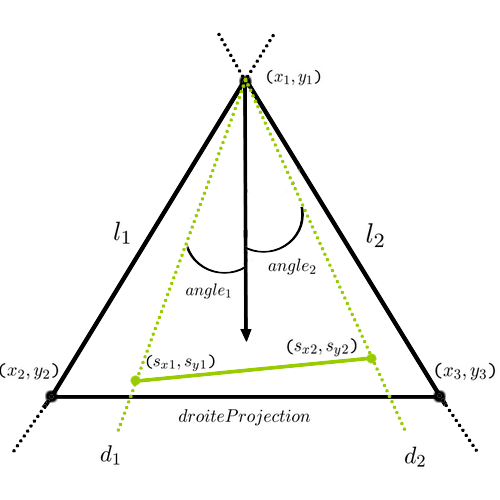
\includegraphics[scale=0.4]{painter_notations_2.png}
\caption{Notations avec segment $s$}
\label{exp_1}
\end{figure}
\newline
\begin{figure}[!h]
\centering
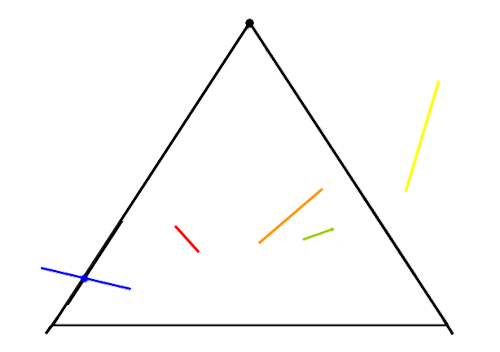
\includegraphics[scale=0.4]{base.png}
\caption{Scène de base}
\label{exp_2}
\end{figure}

Pour chaque segment dans la liste, nous allons déterminer si celui ci est visible par le point de vue (entièrement ou non) et l'afficher si c'est le cas.

Pour chaque segment, nous calculons les droites partant de point de vue et allant jusqu'à ses deux extrémités ainsi que les angles que ces droites forment avec le vecteur directeur. Ces angles nous permettent de déterminer si le segment est bien compris dans la vue ou non. Les droites en poitillé sur la figure \ref{exp_3} montre cette situation (les angles ne sont pas représentés).

\begin{figure}[H]
\centering
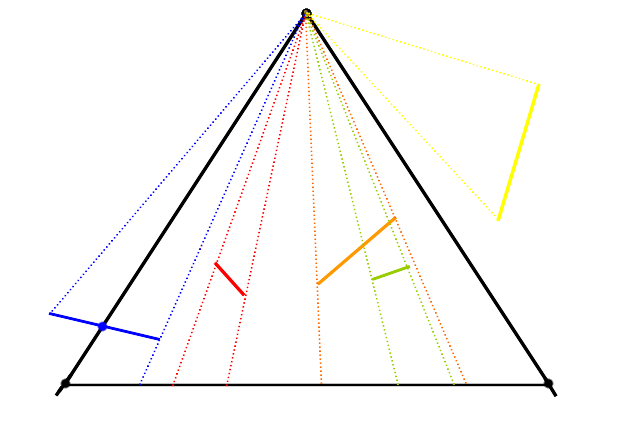
\includegraphics[scale=0.6]{inter.png}
\caption{Scène avec calcul des droites}
\label{exp_3}
\end{figure}

16 à 18 
Si les deux angles sont plus petit que le demis angle, il est évident que le segment est complètement compris dans la vue (fig1) nous l'affichons donc en entier. Pour ce faire nous projetons ses extrémités sur la droite de projection (pointillés) et dessinons le segment reliant ces intersections comme sur la figure \ref{cas1}

\begin{figure}[H]
\centering
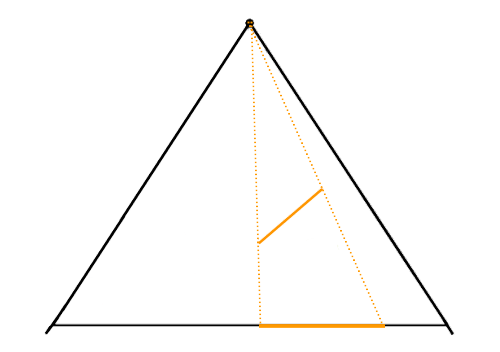
\includegraphics[scale=0.6]{cas1.png}
\caption{Cas du segment complètement dans la projection}
\label{cas1}
\end{figure}

20 à 41
Si un des deux angles est plus grand que le demis angle et l'autre plus petit, nous savons que le point qui compose la droite qvec l'angle a l'intérieur est dans la vue. Nous devons dès lors déterminer l'autre point d'intersection qui se trouve sur la ligne $l_1$ ou 
$l_2$ Pour déterminer cela, nous procédons comme suit :

Nous calculons la position du segment par rapport aux lignes $l_1$ et $l_2$. Si nous obtenons deux intersections, nous avons le cas particulier ou le segment coupe $l_1$ ou $l_2$ devant le point de vue et $l_2$ ou $l_1$ derrière cette situation est représentée sur la figure \ref{exp4}. 

\begin{figure}[H]
\centering
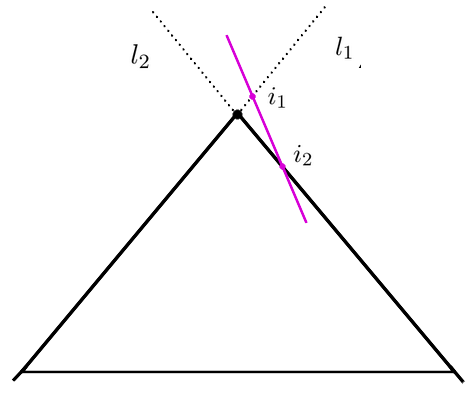
\includegraphics[scale=0.6]{casSpecial1.png}
\caption{cas spécial ou il y a deux intersections}
\label{exp_4}
\end{figure}

Pour déterminer l'intersection qui nous intéresse $i_1$ ou $i_2$ (celle devant le point de vue)  nous calculons la norme allant du point dans la vue jusq'à cette intersection. Il est évident que la norme la plus petite est celle avec la bonne intersection (car être devant le point de vue force à avoir une norme moins grande). Nous savons ainsi si la ligne $l_1$ ou $l_2$ intersecte le segment. LE deuxième point du segment est donc sur cette ligne $l_1$ ou $l_2$ et dans le but de dessiner ce segment, nous en calculons les projections (du point via la technique précédente) et de l'intersection sera une des limites car comme dit précédemment la projection d'un poitn sur $l_1$ ou $l_2$ est respectivement $limite_1$ et $limite_2$

Si nous obtenons qu'on a qu'une seule intersection, la ligne $l_1$ ou $l_2$ qui intersecte nous donne la position de l'intersection et donc de l'autre point $limite_1$ ou $limite_2$. Le segment bleu sur la figure \ref{exp_3} montre cette situation ou l'intersection $i_1$ nous donne un point d'intersection, ce qui nous permet de savoir que la ligne $l_1$ est intersectée. L'angle nous avait permis de savoir que le point ($s_{x_2},s_{y_2}$) du segment bleu $s$ était dans la vue. Le segment a dessiner ira donc de $limite_1$ à la projection de ($s_{x_2},s_{y_2}$) sur le segment de projection comme expliqué sur la figure \ref{cas2}

\begin{figure}[H]
\centering
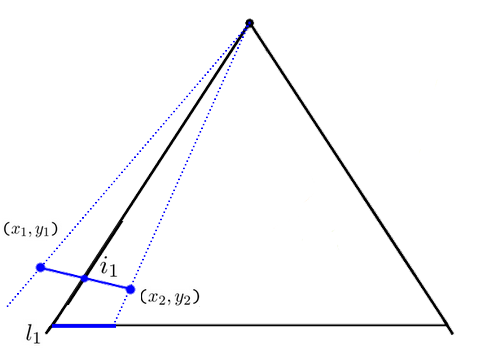
\includegraphics[scale=0.6]{cas2.png}
\caption{Cas ou le segment est coupé par $l_1$}
\label{cas2}
\end{figure}

Enfin, si nous avons deux angles plus grands que demis angle, et qu'on ai une droite de chaque coté (ceci veut dire qu'on a une droite de chaque coté) et qu'on moins une des droites est devant le point de vue, il est possible que le segment coupe complètement le point de vue. Dès lors, nous calculons les interections avec $l_1$ et $l_2$ et si nous obtenosn deux intersections, nous calculons les projections qui sont les deux limites et appellons récursivement la méthode. Ceci débouche sur deux cas :

LE segment était bien devant et les deux angles sont donc inférieurs, le segment est dessiné.
Le segment coupait les deux droites derrière le point de vue, nous repassons dans le dernier cas, mais dorénavant nous n'avons plus d'intersection mais gauche ou droite.

Ces deux cas sont représentés sur les figure \ref{exp_5} et \ref{exp_6}.

\begin{figure}[H]
\centering
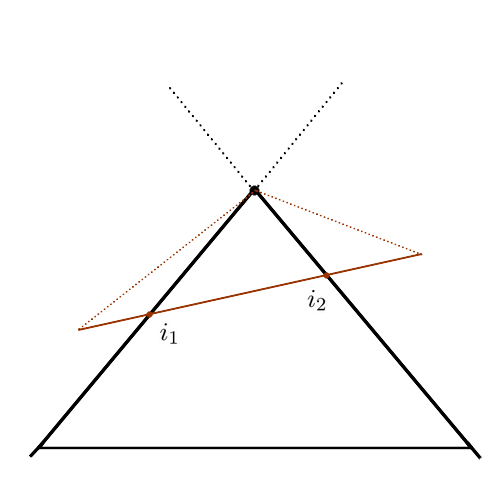
\includegraphics[scale=0.5]{casSpecial2.png}
\caption{cas spécial ou il y a deux intersections devant}
\label{exp_5}
\end{figure}
\subsection{Tests \& Résultats}

\begin{figure}[!h]
\centering
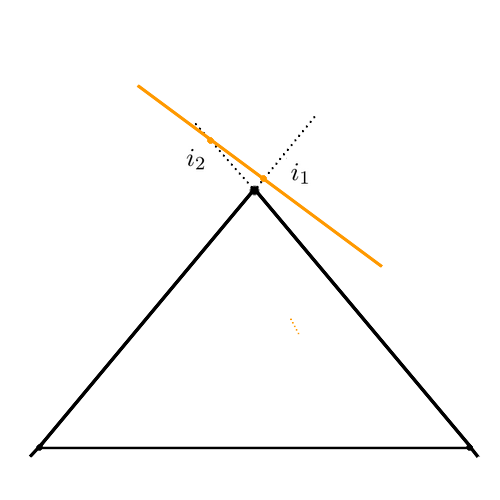
\includegraphics[scale=0.5]{casSpecial3.png}
\caption{cas spécial ou il y a deux intersections derrière}
\label{exp_6}
\end{figure}


\subsection{Tests \& Résultats}
L'algorithme du peintre parcourant tous les noeuds de l'arbre BSP ainsi que tous les segments contenus dans la ligne de séparation de l'espace de ce noeud, il est naturel que le temps d'exécution de l'algorithme dépendra du nombre de noeuds de l'arbre ainsi que du nombre de segments contenus dans l'arbre (la somme du nombre de segments contenus dans chaque noeud). Le tableau suivant nous donne les valeurs de temps pour chaque arbre créé via une heuristique ainsi que le temps pris par l'algorithme du peintre. Il convient aussi de remarquer que plus il y aura de segments contenus dans le point de vue, plus il y aura de calculs effectués par la méthode scanConvert



Nous remarquons que plus le nombre de segments est élevé, plus l'algorithme du peintre prendra du temps.

\section{Mode d'emplois}

\subsection{Interface graphique}

Afin de lancer l'interface graphique, la classe \textit{TestGui.java} du package \textit{be.umons.ac.gui} doit être lancée. 

L'interface graphique fonctionne comme suit :
Lors du lancement de l'interface graphique, il est demandé à l'utilisateur de choisir un fichier contenant une scène et une heuristique de construction de l'arbre. Suite à ce choix, une fenêtre montrant la représentaton de la scène est ouverte. La barre de menu en haut de cette fenêtre permet de choisir un différent fichier ou une heuristique différente. Elle permet aussi de choisi le monde d'input de l'angle de vue.

Mode 1 : Choix manuel : le premier click donne la position du point de vue. Les deux suivants donnent l'angle de vue proprement dit.
Mode 2 : Choix de l'angle : lorsceque ce choix est pris, il est demandé à l'utilisateur d'entrer un angle de vue. Celui ci peut alors clicker deux fois pour donner la droite bisecrite de l'angle de vue.

L'algorithme du peintre est représenté une fois un angle valide choisis par l'utilisateur. Il est représenté deux fois pour une meilleure compréhension : une fois sur une droite directement sur le point de vue et une autre au dessus de la fenête mis à l'échelle et donc plus grande et visible pour les gros fichiers.

\subsection{Mode console}

Pour lancer le mode console, la classe \textit{TestCui.java} du package \textit{be.umons.ac.cui} doit être lancée.

Le mode console fonctionne comme suit :
Il est tout d'abord demandé à l'utilisateur de choisir un fichier. Il doit pour cela introduire le chemin complet de celui-ci dans la console. Suite à cela, les temps de création des arbres via les différentes heuristiques ainsi que les temps d'éxécution de l'algorithme sur peintre sur ces arbres sont affichés sous forme de tableau. Les temps affichés sont en secondes. 

\section*{Conclusion}

\addcontentsline{toc}{section}{Conclusion}
\end{document}